% DATP: Device-Aware Threshold Personalization — A Controlled Threshold-Calibration Study
% IEEE Conference Paper — IEEEtran format
\documentclass[conference]{IEEEtran}
% \IEEEoverridecommandlockouts  % removed: no \thanks{} used in this paper

\usepackage{cite}
\usepackage{amsmath,amssymb,amsfonts}
\usepackage{algorithmic}
\usepackage{graphicx}
\usepackage{textcomp}
\usepackage{xcolor}
\usepackage{booktabs}
\usepackage{multirow}
\usepackage{makecell}
\usepackage{url}
\usepackage{siunitx}
\usepackage{textcase}
\usepackage[hidelinks]{hyperref}

\sisetup{detect-all, round-mode=places, round-precision=4}

% Protect dataset name casing in captions
\newcommand{\CICIoT}{\NoCaseChange{CICIoT2023}}

\def\BibTeX{{\rm B\kern-.05em{\sc i\kern-.025em b}\kern-.08em
    T\kern-.1667em\lower.7ex\hbox{E}\kern-.125emX}}

\begin{document}

\title{Device-Aware Threshold Personalization:\\ A Controlled Threshold-Calibration Study for\\ Non-IID Federated IoT Anomaly Detection}

\author{
\IEEEauthorblockN{Salaheddine Naslouby\IEEEauthorrefmark{1},
Mohamed Lachgar\IEEEauthorrefmark{2},
Hamid Hrimech\IEEEauthorrefmark{3}}
\IEEEauthorblockA{\IEEEauthorrefmark{1}\IEEEauthorrefmark{3}LAMSAD Laboratory, National School of Applied Sciences (ENSA),
Hassan First University, Berrechid, Morocco}
\IEEEauthorblockA{\IEEEauthorrefmark{2}L2IS Laboratory, Higher Normal School (ENS),
University Cadi Ayyad, Marrakech, Morocco}
}

\maketitle

\begin{abstract}
\textbf{Objective:} This study isolates threshold calibration scope as the sole experimental variable in a federated IoT anomaly-detection pipeline. A fixed FedAvg autoencoder ($E{=}1$, full participation) is trained once per seed; the same encoder, seeds, and per-client score artifacts are reused across shared (B1), per-client (B2), family-mean (B3), and cluster-mean (B4) threshold policies---a threshold-only controlled comparison.
\textbf{Protocol:} The primary comparison is B1 vs.\ B2 on N-BaIoT ($K{=}9$ physical devices, $q{=}0.95$, five seeds). Because B2 sets each client's threshold at its own benign $p_{95}$, FPR equalization is expected by construction under stable calibration/test distributions; the empirical contribution is the held-out magnitude, seed consistency, detection-quality tradeoff, and B4's taxonomy-free approximation.
CICIoT2023 (Regime~B) uses randomized file-level pseudo-clients---not physical devices---as a near-homogeneous applicability boundary.
\textbf{Results:} B2 reduces CV(FPR) from 1.017 to 0.299 ($\Delta{=}0.718$, bootstrap CI $[0.647,\,0.769]$, all five seed deltas positive). B4 recovers ${\approx}52\%$ without a taxonomy. The gain is not uniform: lower-tail Macro-F1 degradation concentrates in a single low-separability client. Under the CICIoT2023 partition, no improvement is observed.
\textbf{Limits:} Nine devices; $E{=}1$ limits local drift; five seeds; CICIoT2023 conclusions hold only under the tested randomized partition.
\end{abstract}

\begin{IEEEkeywords}
federated learning, IoT anomaly detection, threshold calibration, false-positive-rate dispersion, autoencoder, non-IID data, personalization.
\end{IEEEkeywords}

\section{Introduction}
\label{sec:introduction}

Federated learning (FL) trains shared models without pooling raw traffic~\cite{mcmahan2017communication}.
Reconstruction-error autoencoders (AEs) are a natural fit for IoT intrusion detection
because benign-only training suffices and attack labels are not required at training time.

A standard deployment trains one shared AE via FedAvg, then applies a threshold $\tau$
above which a reconstruction error signals an intrusion.
In homogeneous fleets this works well.
In heterogeneous fleets, however, benign reconstruction-error distributions differ
substantially across device types: a single shared $\tau$ imposes unequal false-positive
rates (FPRs).
Some devices carry a disproportionate false-alarm burden---making them noisy
or operationally unusable---while others may become under-sensitive.
A shared server-broadcast threshold is natural in deployments where the system
exposes a single global alarm boundary or where per-client threshold state is
not managed independently.

This study asks how large the per-client FPR disparity is under a shared threshold,
how much per-client calibration reduces it, and what detection-quality tradeoff
this creates---all under a fixed FedAvg AE with real physical-device heterogeneity.
The target operational scenario is a fleet of physical IoT devices for which
local benign calibration data are available, and where reducing unequal
false-alarm burden across devices is a deployment priority.
Prior FL-AE work may report aggregate detection metrics or use thresholds implicitly,
but without fixing the encoder, aggregation protocol, and training hyperparameters and
varying only threshold scope, it is impossible to attribute per-client alarm-rate
dispersion to the threshold policy rather than to training differences.
This controlled-comparison gap motivates the present study.

The primary metric is the coefficient of variation of FPR across eligible clients,
$\text{CV(FPR)} = \sigma_{\text{FPR}} / \mu_{\text{FPR}}$.
Four threshold policies are evaluated: a client-averaged shared threshold (B1), full per-client
personalization (B2), device-family grouping (B3), and unsupervised cluster grouping (B4).
B1 is constructed as the arithmetic mean of eligible clients' local 95th-percentile
benign calibration thresholds, broadcast as a single scalar.
The arithmetic mean treats eligible clients equally and models a simple server-broadcast
threshold derived from local calibration summaries, avoiding sample-count domination;
pooled and sample-weighted alternatives are reported as sensitivity checks.
A centralized baseline (B0) is included as a privacy-incompatible reference
comparator but is not part of the single-variable B1--B4 comparison.

The study uses N-BaIoT~\cite{meidan2018n} as the primary confirmatory regime (Regime~A),
CICIoT2023~\cite{neto2023ciciot2023} as a file-level applicability check under
near-homogeneous conditions (Regime~B), and synthetic Dirichlet partitions of N-BaIoT as a
heterogeneity severity sweep (Regime~C).
Five random seeds are used; seed-level descriptive summaries (mean, SD, range, sign consistency) report stability.
The FL simulation uses Flower~\cite{beutel2020flower}.

This article contributes a threshold-only calibration analysis for federated IoT
anomaly detection. It quantifies the false-positive-rate disparity induced by shared
thresholds across heterogeneous physical devices, evaluates per-client, family-mean,
and cluster-mean calibration under a fixed FedAvg autoencoder, characterizes the
resulting detection-quality tradeoff, and provides reproducible source code,
configurations, per-seed results, and figure-generation scripts through an
archived replication artifact.

The remainder of this article is organized as follows. Section~\ref{sec:related}
reviews related FL autoencoder, non-IID aggregation, model-personalization, and
threshold-personalization work; Sections~\ref{sec:formulation}--\ref{sec:experiments}
define the alarm decision, dispersion metric, threshold-personalization framework,
datasets, regimes, and evaluation protocol;
Sections~\ref{sec:results}--\ref{sec:conclusion} report the results, discuss validity
threats, and conclude with practitioner guidance, limitations, and future work.

\section{Related Work}
\label{sec:related}

Federated autoencoders for IoT anomaly detection have been applied to
device-partitioned N-BaIoT by Rey~et~al.~\cite{rey2022federated},
Khraisat~et~al.~\cite{khraisat2025fediot}, and
Olanrewaju~et~al.~\cite{olanrewajugeorge2025flae}, who report aggregate detection
metrics. Thresholds are applied implicitly or globally; none isolates threshold
calibration scope as a variable or measures per-client FPR dispersion.

Non-IID aggregation work such as FedMSE~\cite{nguyen2025fedmse} improves AUC under
Dirichlet non-IID N-BaIoT by changing aggregation weights, not post-training threshold
policy; per-client alarm-rate dispersion is not
reported~\cite{zhao2018noniid,li2022federated}.

Model-level FL personalization methods such as Per-FedAvg, FedPer, and
LG-FedAvg~\cite{fallah2020personalized,arivazhagan2019federated,liang2020think} adapt
weights or training objectives, whereas DATP fixes the shared AE and adapts only the
post-training alarm boundary.

Threshold-level personalization is acknowledged in
Kitsune~\cite{mirsky2018kitsune} and DIoT~\cite{nguyen2019diot}, but neither provides
a controlled comparison fixing encoder, training protocol, and seeds across
threshold-scope variants. Recent FL-AE IoT IDS and non-IID aggregation studies improve aggregate detection or training behavior, but threshold scope remains implicit, fixed, or unvaried; conversely, local-threshold systems acknowledge per-device calibration without isolating it under a frozen federated encoder. Table~\ref{tab:related_comparison} summarizes this gap.

\begin{table}[!b]
  \caption{Positioning: adaptation layer and threshold treatment.}
  \label{tab:related_comparison}
  \centering
  \footnotesize
  \renewcommand{\arraystretch}{1.2}%
  \setlength{\tabcolsep}{4pt}%
  \begin{tabular}{@{}l>{\raggedright\arraybackslash}p{2.3cm}>{\raggedright\arraybackslash}p{2.3cm}@{}}
    \toprule
    Work group & Adaptation layer & Threshold treatment \\
    \midrule
    FL-AE IoT IDS~\cite{rey2022federated,khraisat2025fediot} & Model (shared AE) & Implicit/global \\
    FedMSE~\cite{nguyen2025fedmse} & Aggregation weights & Not varied \\
    Per-FedAvg, FedPer~\cite{fallah2020personalized,arivazhagan2019federated} & Model weights/ objectives & Not addressed \\
    Kitsune, DIoT~\cite{mirsky2018kitsune,nguyen2019diot} & Local AE & Per-device (no controlled study) \\
    \textbf{DATP (this work)} & \textbf{Threshold only} & \textbf{Controlled comparison} \\
    \bottomrule
  \end{tabular}
\end{table}

\section{Problem Formulation}
\label{sec:formulation}

\subsection{Notation}
Let $\mathcal{K}=\{1,\dots,K\}$ denote the set of FL clients.
Each client $k$ holds local benign traffic data $\mathcal{D}_k^{\text{ben}}$ and may have
attack data $\mathcal{D}_k^{\text{atk}}$.
An autoencoder $h = g \circ f$ maps input $\mathbf{x} \in \mathbb{R}^d$ to a reconstruction
$\hat{\mathbf{x}} = g(f(\mathbf{x}))$, where $f$ is the encoder and $g$ the decoder.
The reconstruction error is the per-sample mean squared error:
\begin{equation}
  e(\mathbf{x}) = \frac{1}{d}\|\mathbf{x} - \hat{\mathbf{x}}\|_2^2,
\end{equation}
where $d$ is the input dimension.

\subsection{Binary Alarm Decision}
Given a threshold $\tau_k$ for client $k$, the alarm decision is:
\begin{equation}
  \text{anomaly}(\mathbf{x}) = \mathbf{1}[e(\mathbf{x}) > \tau_k].
\end{equation}
The FPR for client $k$ is $\rho_k = \Pr[e(\mathbf{x}) > \tau_k \mid \mathbf{x} \sim \mathcal{D}_k^{\text{ben}}]$.

\subsection{Dispersion Metric}
Let $\mathcal{K}_{\mathrm{elig}}\subseteq\mathcal{K}$ denote clients with at least $n_{\min}=100$ benign calibration samples; other clients are calibration-pending and excluded from dispersion metrics. The primary metric is the coefficient of variation of FPR over $\mathcal{K}_{\mathrm{elig}}$:
\begin{equation}
  \text{CV(FPR)} = \frac{\sigma_{\rho}}{\mu_{\rho}},\quad
  \mu_{\rho} = \frac{1}{|\mathcal{K}_{\mathrm{elig}}|}\sum_{k\in\mathcal{K}_{\mathrm{elig}}} \rho_k,
\end{equation}
where $\sigma_{\rho}$ is the standard deviation.
CV(FPR) normalizes cross-client FPR dispersion by the fleet mean, making dispersion
comparable across regimes with different mean FPR levels; IQR(FPR) and
max--min FPR are reported as absolute-dispersion checks to guard against small-denominator artifacts.

\textbf{Eligibility and fallback.}
Calibration-pending clients receive the client-averaged shared threshold $\tau_{\text{global}}$ (B1 value) as a fallback. Coverage is reported as $|\mathcal{K}_{\mathrm{elig}}|/|\mathcal{K}|$ for all conditions.

\textbf{Operational assumption.}
Percentile calibration assumes each client's benign reconstruction-error distribution
is sufficiently stable between calibration and test.
Temporal drift would weaken the calibration guarantee; this paper does not model concept drift.

\subsection{Confirmatory Statistic}
The primary statistical estimate is the seed-level delta:
\begin{equation}
  \Delta_s = \text{CV(FPR)}_{\text{B1},s} - \text{CV(FPR)}_{\text{B2},s},
\end{equation}
aggregated over seeds $s \in \mathcal{S}$ via descriptive summaries: mean, standard deviation, range, and sign consistency.
With only five seeds, these statistics are reported as a seed-level consistency summary---not a high-powered
population significance test.
All-positive seed deltas are interpreted as seed-level support
for RQ2 in this tested protocol.

\subsection{Research Questions}
\begin{itemize}
  \item \textbf{RQ1:} Under the client-averaged shared threshold (B1), how large is the variation of FPRs across heterogeneous IoT clients?
  \item \textbf{RQ2:} What held-out FPR-dispersion reduction does per-client threshold calibration (B2) achieve relative to the client-averaged shared threshold under physical-device heterogeneity, what TPR/Macro-F1 tradeoff does this impose, and how much of the per-client benefit does taxonomy-free cluster grouping (B4) recover?
  \item \textbf{RQ3:} How much of the B2 dispersion reduction can cluster-mean calibration (B4) recover?
\end{itemize}

The benign calibration-error distributions of different device types differ substantially
in location and spread, so the B1 client-averaged threshold $\tau_{\text{global}}$ crosses
each distribution at a different fraction, producing device-specific FPRs.
Because B2 uses each client's local benign percentile, FPR equalization is expected
when calibration and test distributions are stable; the empirical questions are therefore
the held-out magnitude of this expected calibration effect, its seed-level consistency,
the detection-quality cost it creates, and the extent to which grouped calibration (B4)
approximates per-client calibration without a device taxonomy---all under a fixed FL-AE
setting with real physical-device heterogeneity.

\section{Threshold Personalization Framework}
\label{sec:framework}

Fig.~\ref{fig:per-device-fpr} illustrates the operational consequence of heterogeneous
calibration: under B1 (client-averaged shared~$\tau$), per-device FPRs vary substantially
across the nine N-BaIoT clients, while B2 (per-client~$\tau$) reduces this dispersion for
the representative seed shown.
As an illustrative preview of the primary Regime~A pattern, Fig.~\ref{fig:per-device-fpr}
shows seed~0 only; inference uses the multi-seed results in Table~\ref{tab:regime_a}.

\begin{figure}[t]
  \centering
  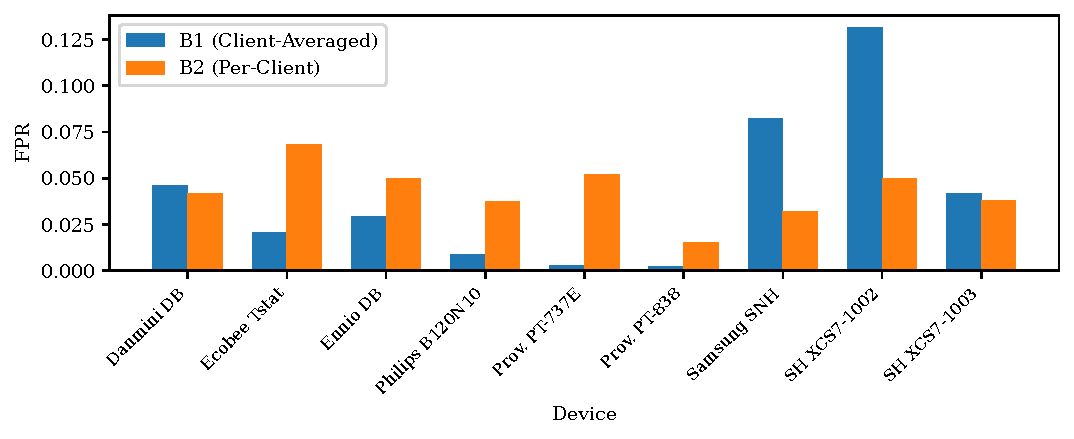
\includegraphics[width=\columnwidth]{figures/figure_1.pdf}
  \caption{Per-device FPR under B1 (Client-Averaged Shared~$\tau$) and B2 (Per-Client~$\tau$)
           for the nine N-BaIoT clients.
           \emph{Illustrative only (seed~0); multi-seed inference uses
           Table~\ref{tab:regime_a} and Table~\ref{tab:per_seed}.}}
  \label{fig:per-device-fpr}
\end{figure}

\begin{figure}[t]
  \centering
  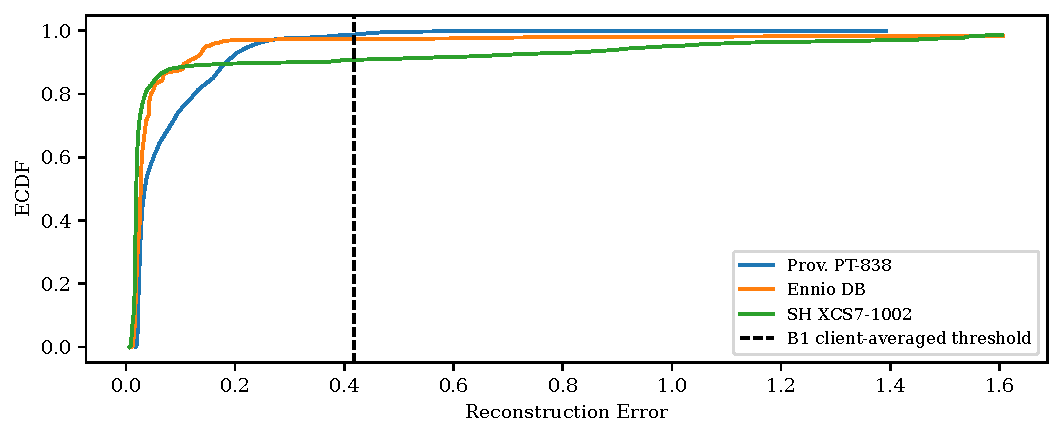
\includegraphics[width=\columnwidth]{figures/figure_2.pdf}
  \caption{Benign reconstruction-error empirical cumulative distributions for three
           representative N-BaIoT clients (seed~0).
           The shared threshold $\tau_{\text{global}}$ (B1, dashed) crosses each curve
           at a different exceedance fraction ($1 - F({\tau})$), producing unequal FPRs.
           Per-client thresholds (B2) set each client's $p_{95}$ independently,
           aligning benign-tail exceedance rates by construction.
           Attack distributions are not shown; they need not shift in parallel with benign tails,
           explaining the TPR/Macro-F1 tradeoff observed in Table~\ref{tab:regime_a}.}
  \label{fig:mechanism}
\end{figure}

\textbf{Pipeline.}
Each client holds benign traffic split into train, calibration, and test partitions;
attack data are reserved exclusively for evaluation and are never used to fit or tune thresholds.
A shared AE is trained with FedAvg via the Flower framework~\cite{beutel2020flower}
(identical training across B1--B4; B0 uses centralized pooling).
\emph{The AE is trained once per (dataset, regime, seed, $\alpha$) condition.}
After training, each client scores its calibration and test data under the fixed AE;
per-client score arrays are written to disk and reused by all threshold policies
without retraining.
Even when a run is budget-capped at 150 rounds, the same final AE state is shared
across all B1--B4 derivations, preserving the threshold-scope-only comparison.

\textbf{Threshold policies.}
Four policies operate on the shared score artifacts:
\begin{itemize}
  \item \textbf{B1 (Client-Averaged):}
        $\tau_{\text{global}} = \frac{1}{|\mathcal{K}_{\mathrm{elig}}|}\sum_{k\in\mathcal{K}_{\mathrm{elig}}} \tau_k^{(95)}$,
        applied uniformly to all clients.
        Pooled and weighted variants are sensitivity checks only
        (Table~\ref{tab:sensitivity_shared}).

  \item \textbf{B2 (Per-Client):} $\tau_k = \tau_k^{(95)}$ applied locally;
        zero additional uplink communication in a deployment where each client
        calibrates its threshold locally.

  \item \textbf{B3 (Family-Mean):} arithmetic mean of local thresholds within each device
        family (Regime~A only; requires a device taxonomy).

  \item \textbf{B4 (Cluster-Mean):} $k$-means on a 4-scalar fingerprint
        $[\mu_e, \sigma_e, \text{skew}_e, p_{95}(e)]$ (StandardScaler-normalized);
        $K{=}3$ for Regime~A, silhouette-selected for Regimes B/C.
        For silhouette selection (Regimes B/C), candidate $K \in \{2,3,4,5\}$;
        $k$-means uses \texttt{k-means++} initialization, $\texttt{n\_init}{=}10$,
        $\texttt{max\_iter}{=}300$, $\texttt{random\_state}{=}42$, applied after
        StandardScaler normalization of the fingerprint matrix.
        The four statistics are compact descriptors of the benign calibration-error
        distribution: $\mu_e$ captures location, $\sigma_e$ spread, $\text{skew}_e$
        tail asymmetry, and $p_{95}(e)$ the operating tail used by thresholding.
        They are distributional summaries for grouping, not privacy mechanisms.
        In Regime~A, $K{=}3$ is a practical fixed choice: with only 9 physical devices
        and coarse device-family structure, silhouette-based $K$ selection is unstable
        at small $n$; $K{=}3$ avoids overfitting cluster count to sampling noise.
        B4 requires sharing these distributional fingerprints, which carries nonzero
        metadata leakage risk (Section~\ref{sec:threats}).
\end{itemize}

Clients with fewer than $n_{\min}{=}100$ benign calibration samples are calibration-pending;
they receive $\tau_{\text{global}}$ as fallback and are excluded from CV(FPR).
\textbf{Evaluation.}
Each client evaluates FPR, TPR, balanced accuracy, and Macro-F1 on held-out test sets.
CV(FPR), CV(TPR), IQR(FPR), worst-client balanced accuracy, $P_{10}$ Macro-F1 (10th percentile
of per-client Macro-F1 across eligible clients), and coverage ratio are aggregated.
Seed-level deltas are summarized descriptively (mean, SD, range, sign consistency).

\section{Experimental Design}
\label{sec:experiments}

\subsection{Datasets and Regimes}

\textbf{Regime A — N-BaIoT (confirmatory).}
The N-BaIoT dataset~\cite{meidan2018n} contains traffic from nine physical IoT devices
grouped by the configured device-family taxonomy, infected with Mirai and BASHLITE botnets.
Each physical device is one FL client ($K=9$).
The N-BaIoT natural partition mixes device-specific benign feature heterogeneity with some
attack-variant skew, and is therefore treated as a realistic natural partition rather than a
pure feature-skew isolation regime.
Regime A is the primary planned condition for RQ2.

\textbf{Regime B --- CICIoT2023 (file-level applicability check).}
CICIoT2023~\cite{neto2023ciciot2023} provides 63 file-defined pseudo-clients under the partition used here.
Regime~B uses randomized file-level pseudo-clients, not physical IoT devices.
Each of the 63 file-defined clients corresponds to one merged flow-level traffic file from the dataset's
\texttt{MERGED\_CSV} directory; client boundaries are defined by the dataset's own
file-level granularity, not by physical device identity.
Within each client, benign records are randomly shuffled (no temporal ordering is preserved)
and split 70/15/15 into train, calibration, and test-benign partitions; attack records
are reserved exclusively for test-attack evaluation.
A per-client cap of 50{,}000 total records is applied, reserving up to 10{,}000 attack records;
this bounds computation and balances benign/attack evaluation volume while preserving
the fixed controlled comparison (after capping, the effective per-client evaluation mix is
approximately 20\% benign and 80\% attack, with median benign count ${\approx}2{,}500$
per client; exact counts are recorded in the replication artifact).
Regime~B tests whether the Regime~A personalization benefit holds when benign
reconstruction-error distributions are near-homogeneous under this partition;
it is not part of the primary B1--B4 comparison.

\textbf{Regime C — Dirichlet non-IID severity (controlled sweep).}
N-BaIoT traffic is repartitioned using a Dirichlet distribution with
$\alpha \in \{0.1,\, 0.3,\, 0.5,\, 1.0,\, 10.0,\, \mathrm{IID}\}$ across $K=20$ synthetic clients.
Lower $\alpha$ means higher heterogeneity.
Regime C provides secondary controlled non-IID severity evidence for the conditions under which threshold personalization is beneficial.

\subsection{Architecture and Training}
The AE encoder has dimensions $[d, 80, 40, 20]$ (ReLU activations, no batch normalization),
where $d=115$ for N-BaIoT and $d=39$ for CICIoT2023.
FL simulation uses the Flower framework~\cite{beutel2020flower} with FedAvg
for up to 150 rounds and a relative-change convergence criterion
(window~$= 10$ rounds, tolerance~$= 0.005$); clients perform $E{=}1$ local epoch
per round with Adam ($\text{lr}=10^{-3}$, batch size 256).
The choice $E{=}1$ keeps training dynamics conservative and fixed while isolating
post-training threshold scope; evaluating larger $E$ is future work because it changes
client drift and reconstruction-error geometry.
With $E{=}1$ and full client participation, FedAvg approaches synchronous distributed
training with frequent aggregation; the FedAvg framing is retained for consistency with
FL-AE literature, and the post-training threshold comparison is invariant to this distinction.
B0 trains a centralized AE on pooled benign data, applying the pooled 95th-percentile
threshold; it is excluded from the B1--B4 controlled ladder.

\subsection{Evaluation Protocol}
Five seeds (0--4) are used. The AE is trained once per seed; B1--B4 thresholds
are derived from shared per-client score artifacts.
The calibration quantile is $q=0.95$;
clients with fewer than $n_{\min}=100$ benign calibration samples are calibration-pending,
receive $\tau_{\text{global}}$ as fallback, and are excluded from CV(FPR).
Budget-capped runs (150 rounds without satisfying the convergence criterion) reuse
the final AE across all B1--B4 derivations, preserving the threshold-only
comparison invariant.
In Regime~A all 5 seeds converged (rounds 51--93);
in Regime~B all 5 were budget-capped;
in Regime~C, 21 of 30 seeds converged (9 budget-capped, concentrated at $\alpha\in\{10.0,\mathrm{IID}\}$).

\subsection{Statistical Analysis}
The primary statistic is the per-seed delta $\Delta_s = \text{CV(FPR)}_{\text{B1},s} - \text{CV(FPR)}_{\text{B2},s}$.
With only five seeds, seed-level descriptive summaries---mean, standard deviation,
range, and sign consistency---are the primary reporting mechanism.
A bootstrap CI (10{,}000 resamples of the five seed-level deltas) is reported as a
supplementary interval estimate; it excludes zero but should be interpreted cautiously
given the small seed count.
Coverage ratio $\rho_{\text{cov}} = |\mathcal{K}_{\mathrm{elig}}| / |\mathcal{K}|$ is reported for all conditions.

Table~\ref{tab:regimes} summarizes the three regimes.
Table~\ref{tab:repro} provides the full reproducibility specification.

\textbf{Environment.}
All experiments ran on a single workstation: AMD Ryzen~5 7600 (6-core), 12\,GB RAM,
NVIDIA GeForce RTX~5060~Ti (16\,GB), Ubuntu~24.04 LTS.
Software: Python~3.12.3, PyTorch~2.11.0 (CUDA~13.0), Flower~1.29.0,
Ray~2.55.0, NumPy~2.4.4, pandas~2.3.3, scikit-learn~1.8.0.
Runtime is not used as an evaluation endpoint in this threshold-scope study.

\begin{table}[t]
  \caption{Experimental Regime Summary}
  \label{tab:regimes}
  \centering
  \footnotesize
  \setlength{\tabcolsep}{5pt}%
  \renewcommand{\arraystretch}{1.2}%
  \begin{tabular}{@{}llcl@{}}
    \toprule
    Regime & Dataset & $K$ & Purpose \\
    \midrule
    A & N-BaIoT & 9 & Confirmatory (B1 vs B2) \\
    B & CICIoT2023 & 63 & Condition-of-applicability check \\
    C & N-BaIoT (Dirichlet) & 20 & Non-IID severity sweep (secondary) \\
    \bottomrule
  \end{tabular}
\end{table}

\begin{table}[t]
  \caption{Reproducibility specification.}
  \label{tab:repro}
  \centering
  \footnotesize
  \renewcommand{\arraystretch}{1.15}%
  \setlength{\tabcolsep}{4pt}%
  \begin{tabular}{@{}lp{0.55\columnwidth}@{}}
    \toprule
    Parameter & Value \\
    \midrule
    AE encoder dims & $[d, 80, 40, 20]$ \\
    Loss / Optimizer & MSE / Adam (lr $10^{-3}$) \\
    Batch size & 256 \\
    Local epochs per round & 1 \\
    Rounds budget & 150 (convergence early-stop) \\
    Convergence criterion & rel.\ change $< 0.005$, window 10 \\
    Client participation & Full (all clients each round) \\
    Normalization scope & Per-client (StandardScaler) \\
    Seeds & $\{0, 1, 2, 3, 4\}$ \\
    Threshold quantile $q$ & 0.95 \\
    Cal.\ eligibility $n_{\min}$ & 100 benign cal.\ samples \\
    N-BaIoT split ratios & 60/20/18 (train/cal/test, gapped)$^{a}$ \\
    CICIoT2023 split & 70/15/15 benign; attack test-only$^{b}$ \\
    CICIoT2023 cap & 50{,}000 total per client (10{,}000 attack) \\
    Score artifact reuse & Train once; B1--B4 from shared scores \\
    \bottomrule
  \end{tabular}
  \par\vspace{2pt}
  \parbox{\columnwidth}{\footnotesize
    $^{a}$ Chronological split with two 1\%-wide temporal gaps to prevent leakage.
    Nominal test fraction~$= 0.18$; gap buffers excluded from all partitions.\\[1pt]
    $^{b}$ CICIoT2023: benign split 70/15/15; attack reserved for test only
    (\texttt{calibration\_benign\_only=True}).
  }
\end{table}

\begin{table*}[!t]
  \caption{Regime~A (N-BaIoT, $K=9$): primary controlled results.}
  \label{tab:regime_a}
  \centering
  \begingroup
  \footnotesize
  \setlength{\tabcolsep}{3pt}%
  \renewcommand{\arraystretch}{1.15}%
  \begin{tabular*}{\textwidth}{@{\extracolsep{\fill}}l c c c c c c c}
    \toprule
    Baseline & Mean FPR & Mean TPR & CV(FPR) & CV(TPR) & Worst~BA & Mean~F1 & P10~F1 \\
    \midrule
    B0 (Centralized)    & $0.057\pm0.001$ & $0.829\pm0.037$ & $0.787\pm0.031$ & $0.278\pm0.036$ & $0.653\pm0.010$ & $0.720\pm0.054$ & $0.403\pm0.059$ \\
    B1 (Client-Averaged) & $0.039\pm0.002$ & $0.738\pm0.050$ & $\mathbf{1.017\pm0.019}$ & $0.289\pm0.029$ & $0.649\pm0.011$ & $0.563\pm0.068$ & $0.344\pm0.062$ \\
    B2 (Per-Client)     & $0.043\pm0.001$ & $0.744\pm0.019$ & $\mathbf{0.299\pm0.073}$ & $0.336\pm0.007$ & $0.651\pm0.001$ & $0.604\pm0.042$ & $0.300\pm0.000$ \\
    B3 (Family-Mean)    & $0.051\pm0.006$ & $0.745\pm0.018$ & $0.964\pm0.096$ & $0.336\pm0.007$ & $0.653\pm0.004$ & $0.606\pm0.038$ & $0.299\pm0.000$ \\
    B4 (Cluster-Mean)   & $0.044\pm0.003$ & $0.718\pm0.019$ & $0.645\pm0.045$ & $0.322\pm0.012$ & $0.654\pm0.007$ & $0.545\pm0.036$ & $0.299\pm0.000$ \\
    \bottomrule
  \end{tabular*}
  \par\vspace{4pt}
  \parbox{\textwidth}{\footnotesize Coverage 9/9, pending 0. Values are mean $\pm$ std over 5 seeds. B0 is a centralized reference and is excluded from the B1--B4 controlled ladder. Worst BA = worst-client balanced accuracy; Mean F1 = mean Macro-F1; P10 F1 = 10th-percentile Macro-F1 across eligible clients.}
  \par\vspace{2pt}
  \parbox{\textwidth}{\footnotesize Primary result: \textbf{B1$-$B2 CV(FPR) $\boldsymbol{\Delta = +0.718}$}, SD$\,{=}\,0.079$, seed range $[0.588,\,0.772]$, all 5 deltas positive; B1$-$B4 $\Delta = +0.372$, SD$\,{=}\,0.055$, seed range $[0.319,\,0.443]$.}
  \endgroup
\end{table*}

\section{Results and Discussion}
\label{sec:results}

\subsection{RQ1: FPR Dispersion Under the Client-Averaged Shared Threshold}

Table~\ref{tab:regime_a} presents aggregate results for Regime~A over 5 seeds.
Under B1, CV(FPR) is $1.017 \pm 0.019$---per-client FPRs vary by more than their mean
(a CV above 1 indicates high relative dispersion).
The natural N-BaIoT B1 CV(FPR) ($1.017$) substantially exceeds the IID Dirichlet
baseline ($0.074$), a difference of $0.943$, consistent with device heterogeneity
contributing to the observed dispersion.
B0's CV(FPR) ($0.787$), although lower than B1's, remains substantially above B2 ($0.299$),
consistent with any single pooled or shared scalar threshold crossing heterogeneous
device-error distributions at different exceedance fractions; B0 is included only as a
centralized privacy-incompatible reference, not as part of the controlled B1--B4 ladder.

Fig.~\ref{fig:regime-a-client-fpr} shows per-client FPR distributions.
The worst client (SimpleHome XCS7 security camera) reaches a mean FPR of approximately
$0.122$ while other clients operate near zero, illustrating the unequal alarm-rate
burden imposed by a single shared threshold across heterogeneous devices.

\subsection{RQ2: Held-Out FPR-Dispersion Reduction and Detection-Quality Cost}

The primary endpoint is the B1 vs.\ B2 CV(FPR) delta per seed.
Across the five planned seeds, the B1--B2 CV(FPR) deltas are all positive,
with mean $\Delta = 0.718$, SD$\,{=}\,0.079$, and range $[0.588,\, 0.772]$
(Table~\ref{tab:per_seed}).
These seed summaries are reported descriptively rather than as confidence intervals.
A supplementary bootstrap CI (10{,}000 resamples of the five seed-level deltas)
yields $[0.647,\, 0.769]$ at 95\%, excluding zero; given five seeds this is
treated as seed-level consistency evidence under the tested protocol.

Per-client calibration (B2) reduces CV(FPR) from $1.017$ to $0.299$ (coverage: 9/9, pending: 0).
B2 reduces CV(FPR) by 0.718 absolute units, corresponding to a relative reduction
$(\mathrm{CV}_{B1}-\mathrm{CV}_{B2})/\mathrm{CV}_{B1}=70.6\%$,
achieved with zero additional threshold uplink.
Operationally, B2 requires local threshold storage, versioning with the encoder/calibration window, and sufficient benign calibration data;
B4 requires transmitting the 4-scalar fingerprint per client.

The tradeoff with detection uniformity is clear from Table~\ref{tab:regime_a}:
CV(TPR) rises under B2 ($0.336$ vs.\ B1's $0.289$),
worst-client balanced accuracy is comparable (B1: $0.649$, B2: $0.651$),
and mean Macro-F1 improves ($0.604$ vs.\ $0.563$).
However, $P_{10}$ Macro-F1 falls from $0.344$ (B1) to $0.300$ (B2).
B2 slightly increases mean FPR ($0.043$ vs.\ $0.039$) but redistributes
false alarms more evenly; B1 attains a lower fleet-average FPR partly by concentrating
false alarms on high-variance clients.
The near-identical P10 Macro-F1 across B2--B4 ($\approx 0.300$, std $< 0.001$)
reflects a floor effect: the Ennio Doorbell client determines the P10 floor
under B2--B4 in all seeds.
Table~\ref{tab:failure_modes} provides the compact client-level separation diagnostic for the two limiting cases: Ennio Doorbell explains the lower-tail Macro-F1 loss under B2, while SimpleHome XCS7 explains the high-FPR tail under B1.

\begin{table}[t]
  \caption{Client-specific separation diagnostics explaining the main lower-tail Macro-F1 and FPR effects (Regime~A, 5-seed averages).}
  \label{tab:failure_modes}
  \centering
  \footnotesize
  \renewcommand{\arraystretch}{1.3}%
  \setlength{\tabcolsep}{4pt}%
  \begin{tabular}{@{}>{\raggedright\arraybackslash}p{1.8cm}>{\raggedright\arraybackslash}p{1.7cm}>{\raggedright\arraybackslash}p{2.0cm}>{\raggedright\arraybackslash}p{2.2cm}@{}}
    \toprule
    Client & Issue & Evidence & Interpretation \\
    \midrule
    SimpleHome XCS7 & Highest FPR under~B1 & Mean FPR ${\approx}\,0.122$ (worst client) & Shared~$\tau$ concentrates false alarms on high-variance devices \\[3pt]
    Ennio Doorbell & P10 Macro-F1 floor under B2--B4 & Lowest AUROC (0.931); 64.9\% attack mass below~$p_{95}$ & Benign/attack overlap limits detection after personalization \\
    \bottomrule
  \end{tabular}
\end{table}

Local thresholding controls Ennio's benign false alarms at the cost of
missing the majority of its low-magnitude attack traffic, explaining the P10 Macro-F1
floor.

\textbf{Mechanism.}
Per-client $p_{95}$ thresholding aligns each client's benign tail, mechanically
equalizing false-alarm rates on benign test traffic.
However, attack reconstruction-error distributions need not shift in parallel
with benign distributions: raising the threshold reduces benign false alarms
but can swallow low-magnitude anomaly scores, reducing TPR or lower-tail
Macro-F1 (Fig.~\ref{fig:mechanism} illustrates the benign-side mechanism).
B2 should therefore be interpreted as an FPR-dispersion calibration policy,
not a uniform detection-quality improvement.

All five seed-level deltas are positive (range $0.588$--$0.772$, Table~\ref{tab:per_seed}).

\begin{table}[t]
  \caption{Per-seed CV(FPR) and deltas, Regime~A.
           All $\Delta_{\text{B1-B2}}$ values are positive.
           B4 recovery $= (\text{B1} - \text{B4}) / (\text{B1} - \text{B2})$.
           Rows are paired by seed, so each B1--B2 delta compares threshold policies on the same frozen AE and score artifacts.}
  \label{tab:per_seed}
  \centering
  \footnotesize
  \renewcommand{\arraystretch}{1.2}%
  \setlength{\tabcolsep}{4pt}%
  \begin{tabular}{cccccc}
    \toprule
    Seed & B1 & B2 & B4 & $\Delta_{\text{B1-B2}}$ & B4 Recov.\ (\%) \\
    \midrule
    0 & 1.045 & 0.347 & 0.632 & $+0.698$ & 59.2 \\
    1 & 1.017 & 0.251 & 0.693 & $+0.765$ & 42.3 \\
    2 & 1.015 & 0.243 & 0.654 & $+0.772$ & 46.6 \\
    3 & 1.018 & 0.251 & 0.575 & $+0.767$ & 57.8 \\
    4 & 0.992 & 0.404 & 0.673 & $+0.588$ & 54.3 \\
    \midrule
    Mean & 1.017 & 0.299 & 0.645 & $+0.718$ & 51.8 \\
    \bottomrule
  \end{tabular}
\end{table}

Absolute FPR dispersion shows the same B1$>$B2 ordering:
IQR(FPR) decreases from $0.035\pm0.002$ (B1) to $0.015\pm0.003$ (B2),
and the max--min FPR gap narrows from $0.120\pm0.007$ to $0.041\pm0.012$.
Because CV(FPR) can be sensitive when mean FPR is small (mean FPR under B1: $0.039$;
under B2: $0.043$), absolute dispersion measures are reported alongside it throughout.
For B1, CV(FPR)$\,{=}\,1.017$ and mean FPR$\,{=}\,0.039$ imply $\sigma_{\text{FPR}} \approx 0.040$;
the CV above~1 therefore reflects genuine cross-client spread comparable to the mean,
not only a small-denominator artifact.

\textbf{Shared-threshold construction sensitivity.}
Pooled and sample-weighted shared-threshold variants preserve the B2 advantage
(Table~\ref{tab:sensitivity_shared}), suggesting the B1-to-B2 reduction is not
driven solely by the arithmetic-mean construction.

\begin{table}[t]
  \caption{Regime~A: shared-threshold construction sensitivity.}
  \label{tab:sensitivity_shared}
  \centering
  \footnotesize
  \setlength{\tabcolsep}{3pt}%
  \renewcommand{\arraystretch}{1.15}%
  \begin{tabular}{@{}llccc c@{}}
    \toprule
    Rule & Construction & CV(FPR) & IQR & \makecell{Max--min\\FPR} & $\Delta$ \\
    \midrule
    B1 & Arith.\ mean & $1.017{\pm.019}$ & $.035{\pm.002}$ & $.120{\pm.007}$ & $+.718$ \\
    B1-pool & Pooled $p_{95}$ & $0.805{\pm.048}$ & $.084{\pm.007}$ & $.134{\pm.012}$ & $+.506$ \\
    B1-wt & Wt.\ mean & $0.907{\pm.033}$ & $.050{\pm.018}$ & $.129{\pm.003}$ & $+.608$ \\
    B2 & Per-client $p_{95}$ & $0.299{\pm.073}$ & $.015{\pm.003}$ & $.041{\pm.012}$ & --- \\
    \bottomrule
  \end{tabular}
  \par\vspace{3pt}
  \parbox{\columnwidth}{\footnotesize Values: mean $\pm$ std, 5 seeds ($q=0.95$). No AE retraining; B1-pool = pooled $p_{95}$; B1-wt = sample-weighted mean of local $p_{95}$. $\Delta$ = vs B2. All B1 variants show larger CV(FPR) than B2, consistent with the advantage not being driven solely by arithmetic-mean construction. B1-pooled has lower CV but higher IQR: raising mean FPR reduces relative dispersion while absolute spread remains larger.}
\end{table}

\begin{figure}[t]
  \centering
  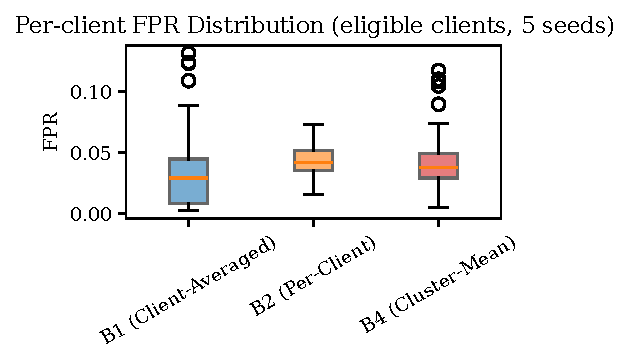
\includegraphics[width=\columnwidth]{figures/figure_3.pdf}
  \caption{Per-client FPR distributions under B1, B2, and B4 (Regime~A, pooled over 5 seeds).
           Descriptive only; inference uses seed-level deltas reported in text.}
  \label{fig:regime-a-client-fpr}
\end{figure}

\subsection{RQ3: Partial Recovery by Cluster-Mean Calibration}

Cluster-mean calibration (B4) achieves CV(FPR) $= 0.645 \pm 0.045$, a partial but consistent improvement over B1.
All five B1$-$B4 deltas are positive (mean $\Delta=0.372$, SD$\,{=}\,0.055$, range $[0.319,\,0.443]$);
all five B4$-$B2 deltas are also positive (mean $\Delta=0.346$, range $[0.269,\,0.442]$).
B4 recovers approximately $52\%$ of B2's improvement (per-seed: $42\%$--$59\%$, Table~\ref{tab:per_seed}).
B4 requires no device taxonomy and transmits only compact 4-scalar fingerprints per client;
however, it does not provide privacy (see Section~\ref{sec:framework}).
Cluster assignments show moderate stability across seeds in Regime~A
(pairwise adjusted Rand index: mean~$0.79$, range $[0.64,\,1.0]$ over all seed pairs).
A post-hoc silhouette check over $K \in \{2,3,4,5\}$ yields mean scores of
$0.29$, $0.31$, $0.34$, and $0.32$ respectively---all low and within $\pm 0.05$---confirming
that the nine-device Regime~A fingerprint space has no clearly dominant cluster count;
$K{=}3$ is a pragmatic fixed choice rather than a structurally optimal partition.
With only nine physical devices, B4 is exploratory and requires validation on larger fleets.
B4's fingerprint still depends on calibration-error statistics including $p_{95}$, so
clients below the eligibility threshold remain calibration-pending and use
$\tau_{\text{global}}$.

Family-mean calibration (B3, Regime~A only) reduces CV(FPR) negligibly
($0.964$ vs.\ B1's $1.017$): the coarse N-BaIoT device-family taxonomy
(Danmini/Ennio doorbells, Ecobee thermostat, Philips baby monitor, Samsung webcam,
Provision/SimpleHome security cameras) does not align with the reconstruction-error
calibration structure---devices within the same family can have dissimilar
benign-error distributions, while devices across families can be similar.
This taxonomy-independence of calibration structure motivates B4's data-driven clustering
over B3's label-based grouping.

\subsection{Regime B: File-Level Applicability Check (CICIoT2023)}

Table~\ref{tab:regime_b} shows Regime~B results.
Under the file-level CICIoT2023 partition, benign reconstruction-error distributions are
near-homogeneous (pairwise JS divergence: mean $0.004$, median $0.003$, max $0.038$
over all $\binom{63}{2}$ pairs and 5 seeds); these low pairwise JS values provide the compact calibration-distribution evidence for the Regime~B near-homogeneity interpretation.
B1 achieves CV(FPR) $= 0.099 \pm 0.002$; B2 increases it to $0.133 \pm 0.007$
(all five seed-level B1$-$B2 deltas are negative; mean $-0.034$, SD $0.006$, range $[-0.043,\,-0.026]$).
When benign distributions are near-homogeneous under this file-level partition, the shared
threshold is already a good fit and per-client calibration introduces variance without
benefit---no personalization improvement was observed in this setting.

\textbf{Interpretation caveat.}
Regime~B uses file-defined CICIoT2023 pseudo-clients (not physical devices) with randomized ordering; it is interpreted only as a near-homogeneous applicability boundary.
Intermediate-round score files are not reported; therefore, Regime~B is interpreted as a controlled threshold-scope check under a shared final frozen AE, with Macro-F1 stable at approximately 0.959 across threshold strategies, not as a convergence-quality claim.

\begin{table*}[t]
  \caption{Regime~B (\CICIoT{} file-defined clients, $K=63$, coverage~63/63, pending~0): mean $\pm$ std over
           5 seeds, eligible clients only. B3 not applicable. All runs budget-capped at 150 rounds.}
  \label{tab:regime_b}
  \centering
  \footnotesize
  \setlength{\tabcolsep}{5pt}%
  \renewcommand{\arraystretch}{1.2}%
  \begin{tabular*}{\textwidth}{@{\extracolsep{\fill}}l c c c c c c}
    \toprule
    Baseline & Mean FPR & Mean TPR & CV(FPR) & CV(TPR) & Worst~BA & Mean~F1 \\
    \midrule
    B0 (Centralized)     & $0.051\pm0.001$ & $0.981\pm0.000$ & $0.109\pm0.020$ & $0.001\pm0.000$ & $0.954\pm0.006$ & $0.959\pm0.000$ \\
    B1 (Client-Averaged) & $0.051\pm0.001$ & $0.982\pm0.000$ & $\mathbf{0.099\pm0.002}$ & $0.001\pm0.000$ & $0.959\pm0.002$ & $0.959\pm0.000$ \\
    B2 (Per-Client)      & $0.051\pm0.001$ & $0.982\pm0.000$ & $0.133\pm0.007$ & $0.001\pm0.000$ & $0.956\pm0.001$ & $0.959\pm0.000$ \\
    B4 (Cluster-Mean)    & $0.051\pm0.001$ & $0.982\pm0.000$ & $0.101\pm0.003$ & $0.001\pm0.000$ & $0.959\pm0.002$ & $0.959\pm0.000$ \\
    \bottomrule
  \end{tabular*}
  \par\vspace{3pt}
  \parbox{\textwidth}{\footnotesize Near-homogeneous regime: pairwise JS divergence mean $0.004$, max $0.038$. B1 achieves lowest CV(FPR); per-client calibration introduces variance without benefit under this partition.}
\end{table*}

\subsection{Regime C: Non-IID Severity Sweep}

Fig.~\ref{fig:severity} and Table~\ref{tab:regime_c} show that the personalization benefit is broadly consistent with larger gains under stronger
heterogeneity, concentrated in the low-$\alpha$ band and absent under near-IID conditions.
Table~\ref{tab:regime_c} reports the corresponding seed ranges, so Fig.~\ref{fig:severity} should be read descriptively rather than as a paired-seed trajectory.
The $\alpha=0.1$ and $\alpha=0.3$ seed ranges overlap ($[0.535,\,0.786]$ vs.\ $[0.420,\,0.897]$),
so strict monotonicity between these two levels should not be inferred from this data;
they form a high-heterogeneity band rather than a strictly ordered pair.
B4 follows the same qualitative pattern but remains a partial approximation.

\begin{figure}[t]
  \centering
  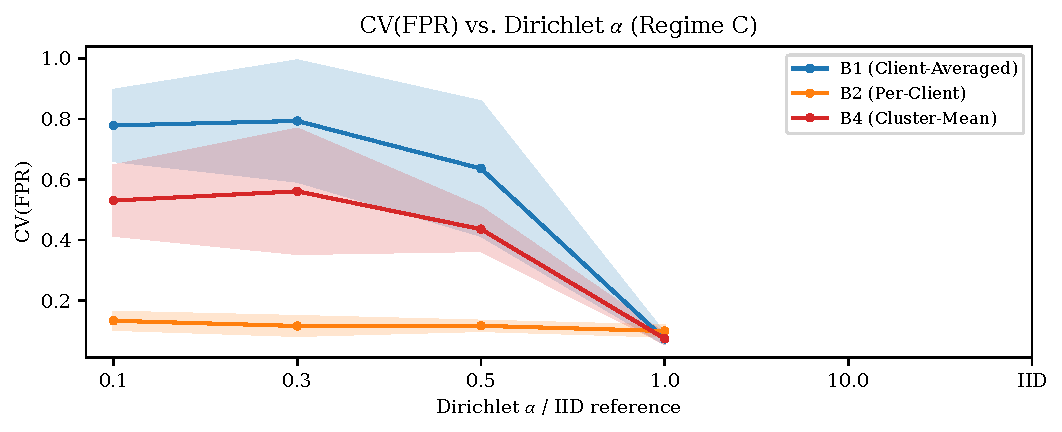
\includegraphics[width=\columnwidth]{figures/figure_4.pdf}
  \caption{Regime C: mean CV(FPR) by threshold strategy as a function of Dirichlet~$\alpha$.
           Whiskers show $\pm$1 std over 5 seeds.
           The B1--B2 gap is largest in the low-$\alpha$ band
           and disappears under IID or near-homogeneous conditions.}
  \label{fig:severity}
\end{figure}

\begin{table}[t]
  \caption{Regime C (N-BaIoT Dirichlet, $K=20$): CV(FPR) sweep.}
  \label{tab:regime_c}
  \centering
  \footnotesize
  \setlength{\tabcolsep}{0.75pt}%
  \renewcommand{\arraystretch}{1.15}%
  \begin{tabular}{@{}l c c c c l@{}}
    \toprule
    $\alpha$ & B1 CV & B2 CV & B4 CV & $\Delta$ & Seed range \\
    \midrule
    0.1  & $.779\pm.104$ & $.134\pm.025$ & $.531\pm.103$ & $0.645$ & $[0.535,\,0.786]$ \\
    0.3  & $.793\pm.178$ & $.117\pm.028$ & $.561\pm.184$ & $0.677$ & $[0.420,\,0.897]$ \\
    0.5  & $.636\pm.197$ & $.117\pm.014$ & $.436\pm.063$ & $0.519$ & $[0.240,\,0.777]$ \\
    1.0  & $.544\pm.116$ & $.096\pm.021$ & $.426\pm.066$ & $0.448$ & $[0.238,\,0.565]$ \\
    10.0 & $.174\pm.053$ & $.111\pm.016$ & $.133\pm.012$ & $0.063$ & $[0.006,\,0.122]$ \\
    IID  & $.074\pm.014$ & $.100\pm.015$ & $.075\pm.013$ & $-0.026$ & $[-0.032,\,-0.019]$ \\
    \bottomrule
  \end{tabular}
  \par\vspace{3pt}
  \parbox{\columnwidth}{\footnotesize Values are mean CV(FPR) $\pm$ std over 5 seeds. Mean FPR $\approx 0.050$ for all levels and baselines. B0 excluded. Coverage 20/20 (pending 0) except $\alpha{=}0.1$ (19--20/20, pending 0--1). $\Delta$\,=\,B1$-$B2 mean delta. Seed range = descriptive min--max over five seeds, not a confidence interval.}
\end{table}

\section{Threats to Validity}
\label{sec:threats}

\textbf{FPR--TPR tradeoff.}
B2 reduces CV(FPR) but increases CV(TPR) ($0.336$ vs.\ $0.289$) and decreases P10 Macro-F1
($0.300$ vs.\ $0.344$); worst-client balanced accuracy is not materially degraded.
In this dataset, the P10 Macro-F1 degradation is concentrated in the low-separability
Ennio Doorbell client (benign-vs-attack AUROC $0.931$, lowest among all nine clients),
so the result is best interpreted as a client-specific failure mode of percentile
calibration rather than evidence of a universal FPR--TPR tradeoff.
Per-client threshold personalization improves false-alarm dispersion fairness, not universal detection quality.

\textbf{Dataset scope.}
Regime~A uses 9 physical IoT devices with natural device-level heterogeneity
(confirmatory); Regime~C ($K{=}20$ synthetic clients) tests severity variation;
Regime~B provides a contrasting near-homogeneous applicability boundary.
The results are a controlled measurement of threshold-scope effects under the tested
protocol, not fleet-scale deployment validation; larger multi-vendor fleets are future work.

\textbf{CICIoT2023 partition.}
Regime~B uses file-level pseudo-clients with randomized within-file benign ordering;
no temporal drift is preserved.
The null result is therefore an applicability boundary under this randomized near-homogeneous
partition only---not evidence that threshold personalization is unnecessary for CICIoT2023
generally.
Chronological, physical-device, attack-source, or attack-type CICIoT2023 partitions would define a different heterogeneity regime and remain outside the present threshold-only controlled comparison.

\textbf{Calibration data sufficiency.}
In all reported conditions, calibration-pending count is zero.
In deployments with fewer than $n_{\min}=100$ benign calibration samples per client,
B2 and B4 fall back to $\tau_{\text{global}}$, reducing their advantage.

\textbf{Threshold quantile sensitivity.}
$q$ is fixed at $0.95$. A sensitivity check over $q \in \{0.90, 0.95, 0.99\}$
preserves the qualitative B2 $<$ B4 $<$ B1 ordering.
The B1-pooled and B1-weighted sensitivity checks are consistent with
the B1-to-B2 gap not being driven solely by arithmetic-mean construction (Table~\ref{tab:sensitivity_shared}).

\textbf{Attack scope and adversarial robustness.}
The evaluation uses Mirai and BASHLITE variants on N-BaIoT.
No poisoning, backdoor, or evasion evaluation is performed.

\textbf{Privacy.}
B4's fingerprint constitutes distributional metadata leakage; B4 is not a privacy mechanism.
Concretely, the mean, variance, skewness, and $p_{95}$ reconstruction-error summaries may
reveal device-specific traffic regularity, tail heaviness, or unusual benign-error profiles;
secure aggregation or noisy aggregation would reduce this metadata exposure.
Mitigations (secure aggregation, differential privacy) are future work.

\textbf{Convergence and budget-capped runs.}
Budget-capped runs limit broad convergence interpretation, but within each seed the
same frozen AE is used across B1--B4, preserving threshold-calibration-only attribution.

\textbf{Architecture and $E{=}1$ scope.}
With $E{=}1$ and full participation, FedAvg approaches synchronous distributed training.
The results characterize threshold-scope personalization under a frequently
synchronized encoder; they should not be read as evidence that the same magnitude
holds under drift-heavy settings ($E>1$ is future work).

\textbf{Concept drift.}
This study uses fixed train/calibration/test splits and does not model online
recalibration; DATP assumes benign reconstruction-error distributions remain
sufficiently stable between calibration and deployment.

\textbf{Seeds and statistical power.}
Five seeds provide limited statistical power.
Seed-level descriptive summaries (all deltas positive, range reported) are appropriate
for this sample size.
All claims are scoped to the tested datasets, partitions, and protocol.

\section{Conclusion}
\label{sec:conclusion}

Under physical-device heterogeneity in N-BaIoT, threshold scope alone strongly changes
the distribution of false alarms across clients: per-client $p_{95}$ calibration (B2)
reduced CV(FPR) from $1.017$ to $0.299$ under the fixed FedAvg AE.
Cluster-mean calibration (B4) recovers $\approx$52\% of B2's improvement without
requiring a device taxonomy, at the cost of transmitting distributional metadata that
is not private; family-mean calibration (B3) performs poorly because coarse device-type
labels do not align with reconstruction-error calibration structure.
Under near-homogeneous conditions (Regime~B file-level CICIoT2023, Dirichlet near-IID)
no dispersion reduction is observed---an applicability boundary, not a general
recommendation against personalization.
B2 is therefore an FPR-equity intervention, not a universal detection-quality improvement:
lower-tail P10 Macro-F1 degradation concentrates in the low-separability Ennio Doorbell
client. Practitioner guidance is therefore two-step: first measure benign calibration-error heterogeneity, using pairwise distribution divergence or dispersion of local calibration thresholds; then choose the threshold policy according to that heterogeneity and deployment constraints. B1 is appropriate when clients are near-homogeneous or per-client state is undesirable; B2 should be considered when local calibration is available and a shared-threshold pilot shows high relative FPR dispersion, for example CV(FPR) near or above~1 with full calibration coverage; B4 is a taxonomy-free compromise when grouping is acceptable, while accounting for metadata leakage from shared distributional fingerprints.

\textbf{Limitations and future work.}
Regime~A uses only 9 physical devices (B4 exploratory at this scale);
Regime~B uses randomized CICIoT2023 file-level pseudo-clients;
$E{=}1$ with full participation limits local drift; five seeds limit statistical power;
no adversarial robustness, formal privacy, or hardware evaluation is provided.
Future work covers larger fleets, $E>1$ sensitivity, privacy-preserving grouping,
model-level personalization, adversarial robustness, and deployment validation under
concept drift.

\textbf{Availability.} Artifact: Zenodo \nolinkurl{10.5281/zenodo.20315654}; release v1.0.0; license and reproduction commands are in the repository.


\bibliographystyle{IEEEtran}
\bibliography{references}

\end{document}
